
\begin{concept}[15cm]
\textit{Nội dung chương này sẽ tập trung trình bày và phân tích, so sánh với các công cụ khác về kết quả mà đề tài đã đạt được sau khi tiến hành thực hiện công việc, kết quả tổng thể mà bộ xử lý đã được đóng góp để hỗ trợ cho hệ thống BE-PUM.}
\end{concept}

\section{Thí nghiệm và đánh giá kết quả}
	\subsection{So sánh với BE-PUM trong quá khứ}
Để thấy được tiến triển của công việc sau quá trình phát triển thêm cho hệ thống BE-PUM, ta sẽ tiến hành chạy thí nghiệm trên một tập 15 malwares ngẫu nhiên với hai phiên bản cũ (trước khi thực hiện công việc) và mới (sau khi thực hiện công việc). Kết quả cần thu thập đó là thời gian thực thi (tính bằng mili giây -- ms), số nút và số cạnh trong đồ thị được sinh ra. Sau đó, ta sẽ tiến hành nhìn nhận và so sánh sự khác biệt giữa trước và sau này.\\

Nhìn vào sự so sánh ở Bảng (\ref{}), ta dễ dàng nhận thấy được số lượng nút và cạnh được BE-PUM dò tìm đã tăng lên một cách rất đáng kể. Đó là nhờ sự hỗ trợ thêm rất nhiều câu lệnh hợp ngữ và Windows API để BE-PUM có thể tính toán và tìm được đường đi trong nội dung của tập tin thực thi. Để dễ dàng thấy được sự chênh lệch này, ta có thể nhìn vào hai biểu đồ ở Hình \ref{fig:exp_comparition_nodes} và Hình \ref{fig:exp_comparition_edges} sau đây.


\begin{figure}[htp]
	\begin{center}
		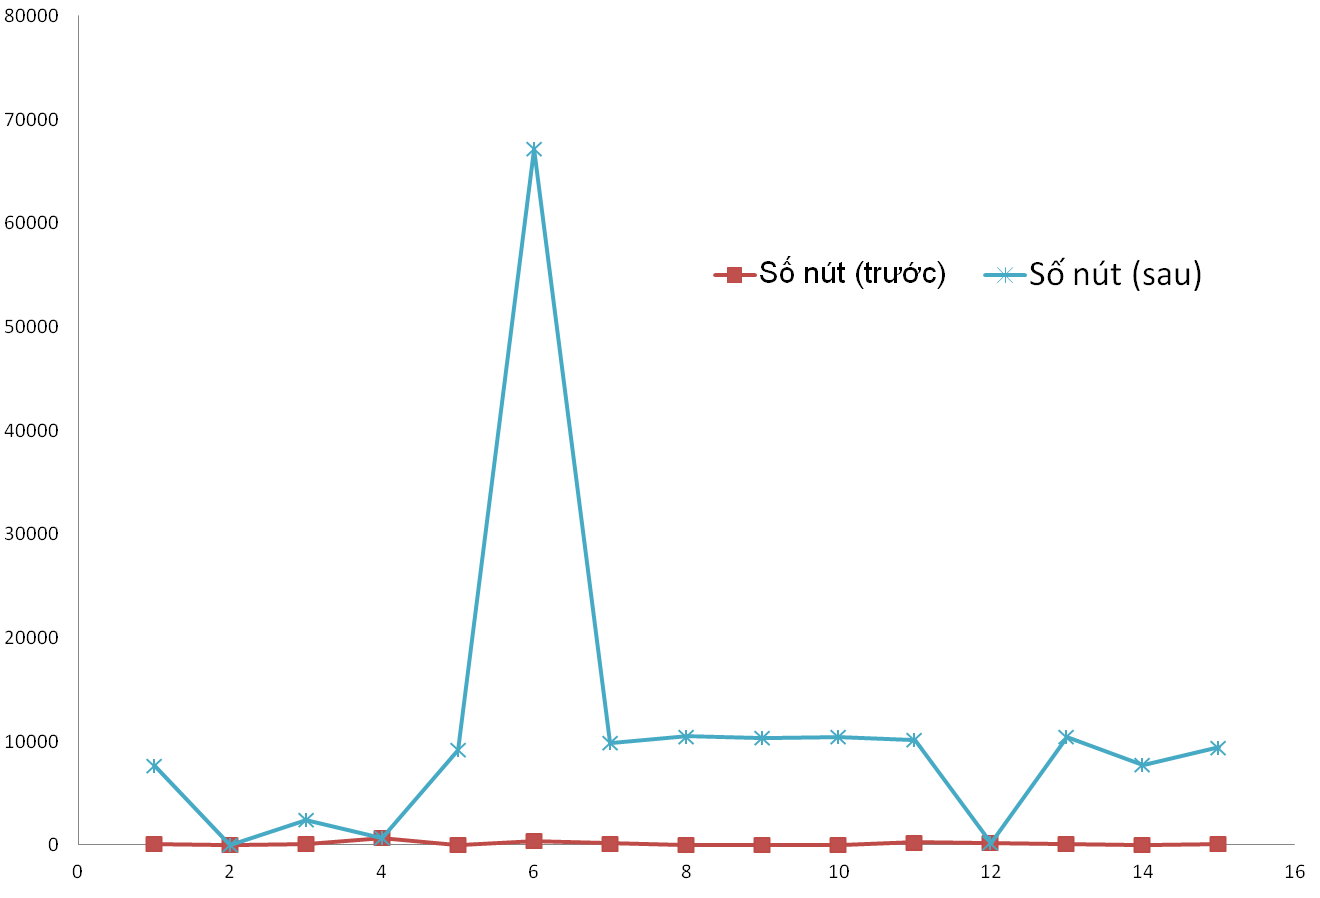
\includegraphics[scale=0.6]{exp_comparition_nodes.png}
	\end{center}
	\caption{Biểu đồ thể hiện số nút của tập thí nghiệm trên hai phiên bản BE-PUM}
	\label{fig:exp_comparition_nodes}
\end{figure}

\begin{figure}[htp]
	\begin{center}
		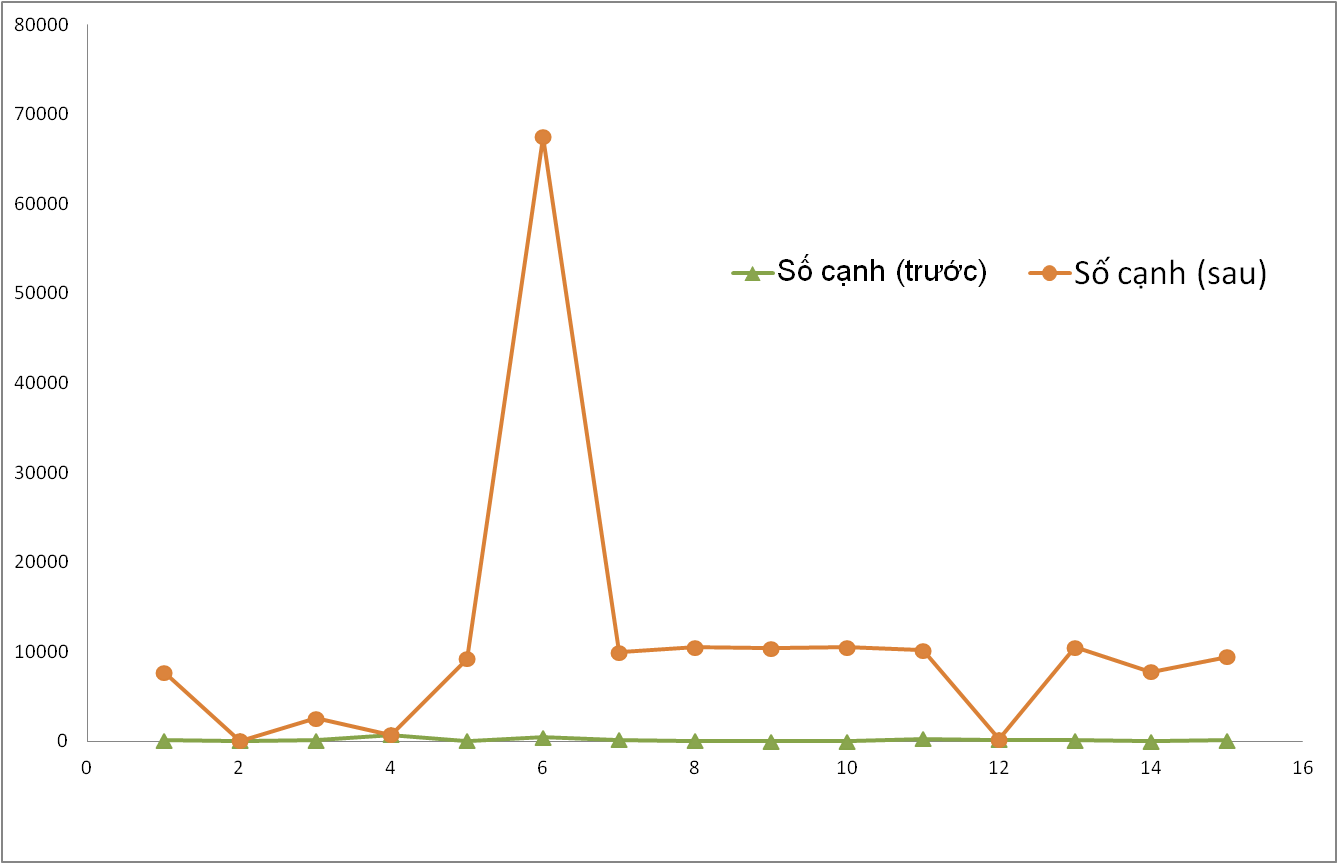
\includegraphics[scale=0.6]{exp_comparition_edges.png}
	\end{center}
	\caption{Biểu đồ thể hiện số cạnh của tập thí nghiệm trên hai phiên bản BE-PUM}
	\label{fig:exp_comparition_edges}
\end{figure}

Bên cạnh việc số lượng các cạnh và nút trong đồ thị tăng lên thì thời gian thực thi cũng tăng lên rất nhiều, do BE-PUM đã phải tính toán nhiều hơn để cho ra được các kết quả đó. Việc này cần được nghiên cứu và giải quyết thêm về sau, khi mà số lượng các thứ BE-PUM hỗ trợ ngày càng bùng nổ.

	\subsection {Kết quả sau cùng}

Sau quá trình thực hiện công việc xây dựng và mở rộng cho hệ thống BE-PUM, toàn bộ phần hiện thực cộng thêm đã được đem ra chạy thí nghiệm trên một tập các malware và không phải malware để đánh giá được khả năng, sức mạnh cũng như những đóng góp mà công việc của luận văn này đã mang lại. \\

Để có được cái nhìn khách quan về BE-PUM, kết quả thí nghiệm sẽ được đem ra so sánh với hai công cụ rất nổi tiếng khác, đó là: \textit{JakStab} và \textit{IDA Pro}.\\

Cả hai công cụ này đều chạy trên phương pháp phân tích tĩnh, nên các trường hợp xử lý phức tạp như \textit{nhảy động} hoặc \textit{tự sửa đổi nội dung mã} sẽ khiến bộ công cụ này thất bại. Nhưng mặt tích cực của phương pháp phân tích tĩnh này là về thời gian xử lý, BE-PUM đánh đổi tiêu tốn nhiều thời gian thực thi \textit{(được tính bằng mili giây -- ms)} hơn nhiều so với đối thủ để hi vọng tìm được nhiều nút và cạnh hơn. Nhìn vào Bảng \ref{table:virusExp}, ta có thể nhận ra ngay được điều đó từ những dòng đầu. \\

Tổng thể kết quả ta có tỷ số giữa số cạnh cùng số nút trong các công cụ JakStab, IDA Pro, và BE-PUM là 1.05, 2.05, và 1.24. Ta thấy được công cụ IDA Pro đã tìm được rất nhiều đường đi trong các tập tin làm ví dụ vì công cụ này hỗ trợ hầu hết các câu lệnh Ntrong khi BE-PUM thì vẫn đang được xây dựng thêm qua công việc của luận văn này. Nhưng có thể đó chỉ là những nhánh không bao giờ được chạy do hạn chế của phân tích tĩnh, không giống như BE-PUM có thể tính toán được giá trị và bỏ đi những nhánh không bao giờ được nhảy tới.

\begin{small}
\setlength\tabcolsep{3pt}
\centering
%\scalebox{0.8}{

\begin{longtable}{|l|l|l|l|l|l|l|l|l|l|l|}
\hline
	\multicolumn{1}{|c}{\multirow{2}{*}{\textbf{Tập tin thực thi}}} & \multicolumn{1}{|c}{\multirow{2}{*}{\textbf{\specialcell{Kích cỡ\\KB}}}} & 
	\multicolumn{3}{|c}{\textbf{JakStab}} & \multicolumn{3}{|c}{\textbf{IDA Pro}} & \multicolumn{3}{|c|}{\textbf{BE-PUM}} \\ \cline{3-11} 
                                   \textbf{} & \textbf{}    & \textbf{Nút}    & \textbf{Cạnh}    & \textbf{Thời gian}   & \textbf{Nút}   & \textbf{Cạnh}   & \textbf{Thời gian} & \textbf{Nút}   & \textbf{Cạnh}   & \textbf{Thời gian}   \\ \hline
                                     
Virus.Artelad.2173	& 23 & 134 & 154 & 10 & 159	& 162	& 1133				& 1610	& 1611	& 236468 \\ \hline
Email-Worm.LoveLetter.b	&	60	&	1027	&	1026	&	297	&	984	&	1011	&	10	&	7558	&	7602	&	1073984	\\ \hline
Virus.Pulkfer.a	&	129	&	907	&	924	&	10	&	805	&	823	&	20	&	8347	&	8353 &	44672	\\ \hline
Email-Worm.Klez.h	&	137	&	192	&	178	&	20	&	50	&	56	&	1	&	5652	&	5651	&	46344	\\ \hline
\hline

Email-Worm.Coronex.a	&	12	&	26	&	27	&	500	&	148	&	157	&	204	&	308	&	339	&	1000 \\ \hline
Trojan-PSW.QQRob.16.d	&	25	&	89	&	100	&	766	&	17	&	15	&	382	&	91	&	105	&	953	\\ \hline
%Virus.Aidlot	&	8	&	81	&	81	&	281	&	64	&	62	&	119	&	105	&	108	&	70344	\\ \hline
Virus.Aztec	&	8	&	104	&	111	&	1973	&	223	&	215	&	495	&	300	&	313	&	44384	\\ \hline
Virus.Belial.a	&	4	&	41	&	42	&	407	&	118	&	116	&	198	&	128	&	134	&	985	\\ \hline
%Virus.Belial.b	&	4	&	43	&	44	&	406	&	118	&	116	&	197	&	139	&	146	&	906	\\ \hline
%Virus.Belial.d	&	4	&	6	&	5	&	328	&	147	&	150	&	158	&	163	&	170	&	1062	\\ \hline
Virus.Benny.3219.a	&	8	&	138	&	153	&	890	&	599	&	603	&	415	&	149	&	164	&	2438	\\ \hline
%Virus.Benny.3219.b	&	12	&	42	&	47	&	453	&	745	&	760	&	200	&	149	&	164	&	2375	\\ \hline
Virus.Benny.3223	&	12	&	42	&	47	&	328	&	770	&	781	&	135	&	149	&	164	&	2218	\\ \hline
Virus.Bogus.4096	&	38	&	87	&	98	&	546	&	88	&	86	&	269	&	88	&	98	&	656	\\ \hline
Virus.Brof.a	&	8	&	17	&	17	&	343	&	98	&	102	&	167	&	137	&	147	&	1484	\\ \hline
Virus.Cerebrus.1482	&	8	&	6	&	5	&	156	&	164	&	165	&	70	&	179	&	198	&	735	\\ \hline
Virus.Compan.a	&	8	&	25	&	26	&	360	&	83	&	81	&	176	&	91	&	98	&	484	\\ \hline
%Virus.Compan.b	&	8	&	21	&	22	&	328	&	68	&	71	&	160	&	83	&	86	&	391	\\ \hline
Virus.Cornad	&	4	&	21	&	20	&	141	&	68	&	72	&	67	&	94	&	100	&	344	\\ \hline
Virus.Eva.a	&	8	&	14	&	13	&	329	&	381	&	392	&	145	&	249	&	277	&	13438	\\ \hline
%Virus.Eva.b	&	12	&	14	&	13	&	172	&	549	&	553	&	59	&	229	&	252	&	3515	\\ \hline
%Virus.Eva.c	&	8	&	14	&	13	&	188	&	448	&	451	&	72	&	292	&	321	&	32532	\\ \hline
%Virus.Eva.d	&	8	&	14	&	13	&	156	&	377	&	381	&	59	&	245	&	272	&	11109	\\ \hline
%Virus.Eva.e	&	20	&	14	&	13	&	204	&	449	&	456	&	80	&	293	&	321	&	15375	\\ \hline
%Virus.Eva.f	&	8	&	14	&	13	&	187	&	350	&	361	&	76	&	204	&	225	&	3672	\\ \hline
%Virus.Eva.g	&	8	&	14	&	13	&	188	&	410	&	421	&	74	&	240	&	261	&	3860	\\ \hline
Virus.Htrip.a	&	8	&	10	&	10	&	359	&	145	&	143	&	172	&	148	&	157	&	2187	\\ \hline
%Virus.Htrip.b	&	8	&	10	&	10	&	343	&	144	&	142	&	164	&	149	&	157	&	2250	\\ \hline
Virus.Htrip.d	&	8	&	10	&	10	&	265	&	164	&	162	&	124	&	165	&	173	&	2296	\\ \hline
Virus.Seppuku.1606	&	8	&	131	&	136	&	1968	&	381	&	390	&	965	&	339	&	364	&	8372	\\ \hline
Virus.Wit.a	&	4	&	54	&	60	&	360	&	153	&	151	&	172	&	185	&	203	&	2641	\\ \hline
%Virus.Wit.b	&	4	&	7	&	7	&	203	&	168	&	166	&	93	&	197	&	214	&	2000	\\ \hline
%Virus.Win9x.I13.b	&	12	&	37	&	37	&	313	&	239	&	240	&	145	&	239	&	245	&	890	\\ \hline
%Virus.Win9x.I13.c	&	8	&	37	&	37	&	172	&	117	&	115	&	80	&	117	&	116	&	500	\\ \hline
%Virus.Win9x.I13.f	&	8	&	41	&	41	&	188	&	131	&	137	&	87	&	131	&	141	&	422	\\ \hline
%Virus.Win9x.I13.h	&	14	&	41	&	41	&	203	&	238	&	242	&	95	&	238	&	258	&	4891	\\ \hline
\hline 

Email-Worm.Bagle.af	&	21	&	123	&	143	&	937	&	142	&	151	&	461	&	140	&	166	&	2157	\\ \hline
Email-Worm.Bagle.ag	&	17	&	127	&	147	&	828	&	13	&	12	&	413	&	127	&	147	&	1047	\\ \hline
%Email-Worm.Bagle.ah	&	22	&	2	&	1	&	203	&	37	&	36	&	100	&	38	&	38	&	297	\\ \hline
%Email-Worm.Bagle.ai	&	21	&	2	&	1	&	109	&	36	&	34	&	53	&	38	&	38	&	218	\\ \hline
%Email-Worm.Bagle.bf   &   30  &   2   &   1   &    3  &   50  &   46  &   89  &   38  &   38  &   189  \\ \hline
\hline 

Virus.Cabanas.a	&	8	&	3	&	2	&	156	&	1	&	1	&	78	&	68	&	72	&	1532	\\ \hline
Virus.Cabanas.b	&	8	&	3	&	2	&	140	&	9	&	7	&	70	&	63	&	66	&	1781	\\ \hline
Virus.Canabas.2999 &      8       &       2       &	1	&	656	&       7	&	6	&	85	&       358	&	401	&	8703	\\ \hline 
\hline 

%Virus.Savior.1740	&	10	&	102	&	113	&	9203	&	99	&	97	&	572	&	202	&	229	&	22953	\\ \hline
%Virus.Savior.1832	&	10	&	102	&	113	&	9438	&	620	&	618	&	688	&	228	&	255	&	23625	\\ \hline
Virus.Seppuku.1638	&	8	&	139	&	144	&	2266	&	414	&	412	&	112	&	689	&	712	&	13000	\\ \hline
Virus.Seppuku.3291	&	8	&	26	&	25	&	187	&	556	&	554	&	66	&	253	&	270	&	12156	\\ \hline
Virus.Seppuku.3426	&	8	&	27	&	27	&	188	&	30	&	28	&	61	&	299	&	317	&	13484	\\ \hline
\hline

\multicolumn{11}{|c|}{\it non-malware binary}  \\ \hline
hostname.exe	& 8 & 329	& 360 &	2412 &    343 &	389 & 	33 & 326 &  357 & 	235610 \\ \hline
winver.exe	& 6 & 162	& 166 &	422 &	310 &	345 &	24 & 232 &  240 &	122484 \\ \hline
%cmd.exe	        & 389 & 168	& 178 &	56 &	500 & 	512 &	0.0342 & 484 &	493 &	273 \\ \hline
systray.exe	& 4 & 110	& 136 & 532 &	115 & 	138 &	14 & 123 &	139 &	16125 \\ \hline
regedt32.exe	& 3 & 52	& 54  &	266 &	56  &	61  & 	11 & 61  &	69  &	22844 \\ \hline
actmovie.exe	& 4 & 164	& 179 &	281 &	187 & 	215 & 	51 & 180 &	196 &	243469 \\ \hline
nddeapir.exe	& 4& 164	& 179 &	500 &	187 & 	215 & 	24 & 180 &	196 &	223297 \\ \hline
%calc.exe	& 114 & 121	& 134 & 28 &	400 &	421 & 	0.0245 & 355 &	373 &	117 \\ \hline
%fixmapi.exe	& 3& 32	& 35  &	42 &	36  & 	45  & 	0.0071 & 43  &	45  &	26 \\ \hline

\caption {Một số kết quả của thí nghiệm sinh mô hình}\label{table:virusExp}
\end{longtable}
%}
\end{small}


		\section{Các câu lệnh hợp ngữ đã được hỗ trợ}
		Trong quá trình mô phỏng các câu lệnh assmebly có sự chọn lọc và ưu tiên các câu lệnh được sử dụng phổ biến trước. Với rất nhiều câu lệnh assembly trong ngôn ngữ cấp thấp được phân ra thành hai nhóm dựa trên thao tác xử lý của câu lệnh bao gồm bộ xử lý số nguyên và bộ sử lý số thực. \\ 
		
	Tính tới thời điểm của bài báo cáo này, đã có khoảng 200 câu lệnh xử lý số nguyên và khoảng 50 câu lệnh xử lý số thực được mô phỏng trong BE-BUM. Bảng ~\ref{tb:ThongKeAss} thống kê danh sách câu lệnh assembly đã mô phỏng được. 
	\begin{longtable}{|m{2cm}|m{3cm}|m{9cm}|}
		\hline
			\multicolumn{2}{|l|}{Bộ xử lý} & Câu lệnh assembly \\
		\hline
		\hline		
			Bộ xử lý số nguyên & Lệnh toán học & ADD, AND, SUB, OR, XOR, IMUL, ROR, DIV, SBB, CLC, NOT, IDIV, XADD, ADC, DEC, SHR, SAR, SHL, SAL, DEC, INC, SHR, ROR, REP, MUL, SAR, RCR, ROL, RCL, SBB \\
		\cline{2-3}
			& Lệnh gọi & CALL \\
		\cline{2-3}
			& Lệnh điều kiện nhảy & JE, JNZ, JC, JC, JLE, JGE, JGE, JLNLE, JS, JNO, JMP, LOOP, JZ, JB, JNB, JNG, JA, JNL, JO, JNS, JNO, JPE, LOOPE, LOOPZ, JNE, JNAE, JAEM JNAEM JL, JNBE, JG, LOOP, JP, JECXZM LOOPNE, LOOPNZ \\
		\cline{2-3}
			& Lệnh nhảy & JUMP\\
		\cline{2-3}
			& Lệnh sao chép& MOV, XCHG, MOVZ, MOVSB, MOVSW, MOSX, MOVZB, MOVZW, CMOVA, CMOVB, CMOVBE, CMOVC, CMOVE, CMOVP, CMOVPE, CMOVG, CMOVL, CMOVNA, CMOVNAE, CMOVNBE, CMOVNE, CMOVNG, CMOVNGE, CMOVNL, CMOVNLE, CMOVNO, CMOVNS, CMOVNZ, CMOVPO, CMOVZ \\
		\cline{2-3}
			& Lênh trả giá trị& RET\\
			\cline{2-3}
			& Lênh điều khiển&CMP, INT, AAA, AAD, AAM, ASS, BSF, BSWAP, BT, BTC, BRT, BTS, CBW, CDQ, CLC, CLD, CLI, CLTD, CMC, OUT, POP, POPA, POPF, PUSH, PUSHA, PUSHF, RDTSC, SAHF, SCAS, SETA, SETAE, SETB, SETBE, SETC, SETE, SETG, SETGE, SETL, SETNA, SETNAE, SETNB, SETNBE, SETNC, SETNE, SETNG, SETNGE, SETNL, SETNLE, SETNO, SETNP, SETNS, SETO, SETP, SETPE, SETPO, SETS, SETZ, LODS, MOVS, NEG, NOP, SHLD, SHRD, STC, STOS, TEST, XLAT, CBW, CWDE, CMPS, CMPXCHG, CMPXCHG8B, CPUID, CWD, CWDE, CWT, DAA, DAS, ENTER, IN INT1, INT3, LAHF, LEA, LEAVE \\
		\hline
			Bộ xử lý số thực & Lệnh toán học &FADD, FADDP, FIADD, FSUB, FSUBP, FSUBR, FSUBRP, FISUB, FISUBR, FMUL, FMULP, FIMUL, FDIV, FDIVP, FIDIV, FDIVR, FDIVRP, FIDIVR, FABS, FCHS, FSQRT, FPREM, FPREM1, FRNDINT, FXTRACT, FSIN, FCOS, FSINCOS, FPTAN, FPATAN, FYL2X, FYL2XP1, F2XM1, FSCALE \\
			\cline{2-3}
			& Lệnh so sánh & FCOM, FCOMP, FCOMPP, FUCOM, FUCOMP, FUCOMPP, FICOM, FICOMP, FCONI, FCOMIP, FUCOMI, FUCOMIP, FTST, FXAM\\
			\cline{2-3}
			& Lệnh nạp giá trị& FLDZ, FLD1, FLDPI, FLDL2T, FLDL2E, FLDLG2, FLDLN2\\
			\cline{2-3}
			& Lệnh sao lưu &FLD, FST, FSTP, FXCH, FCMOVcc, FCMOVB, FCMOVNB, FCMOVE, FCMOVNE, FCMOVBE, FCMOVNBE, FCMOVU, FCMOVNU. \\
			\cline{2-3}
			& Lệnh điều khiển & FINIT, FNINIT, FLDCW, FSTCW, FNSTCW, FSTSW, FNSTSW, FCLEX, FNCLEX, FLDENV, FNSTENV, FRSTOR, FSAVE, FNSAVE, FINCSTP\\
		\hline
		\caption{Thống kê các câu lệnh assembly đã được hiện thực}
		\label{tb:ThongKeAss}
	\end{longtable}
	
\section{Các Windows API đã được hỗ trợ}

Quá trình xây dựng có sự chọn lọc và ưu tiên cho các Windows API được dùng phổ biến trước tiên. Với rất nhiều Windows API của dịch vụ nền được các phần mềm độc hại cho máy tính sử dụng (được chứa bên trong tập tin kernel32.dll), đây là bộ thư viện đang được ưu tiên hỗ trợ hàng đầu cho hệ thống BE-PUM. Kế tiếp đó là các bộ thư viện giao diện người dùng (được chứa bên trong tập tin user32.dll), dịch vụ nâng cao (được chứa bên trong tập tin advapi32.dll) và cuối cùng là Windows Shell (được chứa bên trong tập tin shell32.dll).\\

Tính đến thời điểm của bài báo cáo này, đã có tất cả khoảng 400 Windows API được xây dựng và hỗ trợ cho hệ thống BE-PUM. Chi tiết về các tên hàm Windows API đã có trong BE-PUM được liệt kê trong Bảng \ref{table:tblWapiResult} sau đây.


\begin{longtable}[H]{ | m{3.5cm} | m{10cm} | }

\hline
	Tên tập tin thư viện & Các Windows API đã được hiện thực\\
\hline
\hline

advapi32.dll &
CryptAcquireContext, CryptCreateHash, CryptDecrypt, CryptDeriveKey, CryptDestroyHash, CryptDestroyKey, CryptHashData, CryptReleaseContext, IsValidAcl, OpenProcessToken, OpenThreadToken, RegCloseKey, RegCreateKeyEx, RegOpenKey, RegOpenKeyEx, RegQueryValueEx, RegSetValueEx \\
\hline
comctl32.dll &
InitCommonControls \\
\hline
gdi32.dll &
AddFontResource, AnimatePalette, CreateCompatibleDC, CreatePalette, DeleteObject, DPtoLP, GdiFlush, GdiGetBatchLimit, GetBkColor, GetDeviceCaps, GetStockObject, SetBkColor, SetTextAlign, StrokeAndFillPath, StrokePath \\
\hline
kernel32.dll &
AreFileApisANSI, CloseHandle, CompareFileTime, CompareString, CopyFile, CreateDirectory, CreateEvent, CreateFile, CreateFileMapping, CreateMutex, CreateProcess, CreateRemoteThread, CreateThread, CreateToolhelp32Snapshot, DecodePointer, DeleteCriticalSection, DeleteFile, DeviceIoControl, DisableThreadLibraryCalls, DuplicateHandle, EncodePointer, EnterCriticalSection, EnumDateFormats, ExitProcess, ExitThread, FileTimeToSystemTime, FindAtom, FindClose, FindFirstFile, FindNextFile, FindResource, FlsAlloc, FlsGetValue, FlsSetValue, FlushInstructionCache, FormatMessage, FreeEnvironmentStrings, FreeLibrary, GetAclInformation, GetACP, GetAtomName, GetCommandLine, GetComputerName, GetConsoleCP, GetConsoleMode, GetCPInfo, GetCPInfoEx, GetCurrentDirectory, GetCurrentProcess, GetCurrentProcessId, GetCurrentThread, GetCurrentThreadId, GetDateFormat, GetDiskFreeSpace, GetDiskFreeSpaceEx, GetDriveType, GetEnvironmentStrings, GetEnvironmentVariable, GetExitCodeProcess, GetFileAttributes, GetFileSize, GetFileTime, GetFileType \\

\hline
kernel32.dll & GetFullPathName, GetLargestConsoleWindowSize, GetLastError, GetLocaleInfo, GetLocalTime, GetLogicalDrives, GetLogicalDriveStrings, GetModuleFileName, GetModuleHandle, GetModuleHandleEx, GetNativeSystemInfo, GetOEMCP, GetPriorityClass, GetProcAddress, GetProcessHeap, GetProcessId, GetProcessVersion, GetShortPathName, GetStartupInfo, GetStdHandle, GetStringTypeA, GetStringTypeW, GetSystemDefaultLCID, GetSystemDefaultUILanguage, GetSystemDirectory, GetSystemInfo, GetSystemTime, GetSystemTimeAsFileTime, GetTempFileName, GetTempPath, GetThreadLocale, GetThreadPriority, GetTickCount, GetUserDefaultLangID, GetUserDefaultLCID, GetVersion, GetVersionEx, GetVolumeInformation, GetWindowsDirectory, GlobalAlloc, GlobalFindAtom, GlobalFree, GlobalGetAtomName, GlobalLock, GlobalMemoryStatus, HeapAlloc, HeapCreate, HeapDestroy, HeapFree, HeapReAlloc, HeapSize, InitializeCriticalSection, InitializeCriticalSectionAndSpinCount, InterlockedDecrement, InterlockedExchange, InterlockedIncrement, IsBadReadPtr, IsBadWritePtr, IsDBCSLeadByte, IsDebuggerPresent, IsProcessorFeaturePresent, IsValidCodePage, IsWow64Process, LCMapString, LeaveCriticalSection, LoadLibrary, LoadLibraryEx, LoadResource, LocalAlloc, LocalFree, LocalLock, LocalReAlloc  \\

\hline
kernel32.dll & LockResource, lstrcat, lstrcmp, lstrcmpi, lstrcpy, lstrcpyn, lstrlen, MapViewOfFile, MoveFile, MoveFileEx, MulDiv, MultiByteToWideChar, OpenEvent, OpenFile, OpenFileMapping, OpenMutex, OpenProcess, OpenThread, OutputDebugString, Process32First, Process32Next, QueryPerformanceCounter, QueryPerformanceFrequency, ReadFile, ReadProcessMemory, RegisterWowExec, ReleaseMutex, RemoveDirectory, ResumeThread, RtlUnwind, RtlZeroMemory, SearchPath, SetConsoleCtrlHandler, SetCurrentDirectory, SetEndOfFile, SetErrorMode, SetEvent, SetFileAttributes, SetFilePointer, SetFileTime, SetHandleCount, SetLastError, SetPriorityClass, SetThreadLocale, SetThreadPriority, SetTimer, SetUnhandledExceptionFilter, SizeofResource, Sleep, SuspendThread, SystemTimeToFileTime, TerminateProcess, TerminateThread, Thread32First, Thread32Next, TlsAlloc, TlsFree, TlsGetValue, TlsSetValue, UnhandledExceptionFilter, UnmapViewOfFile, VirtualAlloc, VirtualAllocEx, VirtualFree, VirtualProtect, VirtualProtectEx, VirtualQuery, WaitForSingleObject, WaitNamedPipe, WideCharToMultiByte, WinExec, WriteFile, WritePrivateProfileString, WriteProcessMemory, wsprintf, \_lclose, \_lcreat, \_llseek, \_lopen \\
\hline
mscoree.dll &
\_CorExeMain \\
\hline
msvcrt.dll &
atexit, calloc, fclose, fopen, fprintf, fread, free, fwrite, isalpha, is\_wctype, malloc, memcpy, memmove, memset, remove, srand, strncat, strncmp, strrchr, strstr, time, \_cexit, \_chkesp, \_controlfp, \_except\_handler3, \_fpreset, \_initterm, \_itoa, \_itow, \_ltoa, \_mbsrchr, \_setmode, \_strcmpi, \_\_getmainargs, \_\_p\_\_commode, \_\_p\_\_environ, \_\_p\_\_fmode, \_\_p\_\_\_initenv, \_\_set\_app\_type \\
\hline
ntdll.dll &
NtCreateSection, NtProtectVirtualMemory, NtQueryInformationProcess, NtWriteVirtualMemory \\
\hline
ole32.dll &
CoCreateGuid, CoFileTimeNow, OleInitialize, OleUninitialize \\
\hline
shell32.dll &
ShellAbout, ShellExecute, SHGetFileInfo, SHGetSpecialFolderPath, StrChrI \\
\hline
shlwapi.dll &
PathFindFileName, PathUndecorate \\
\hline
user32.dll &
AnyPopup, BlockInput, CharLower, CharNext, CharPrev, CharUpperBuff, ClientToScreen, CloseWindow, CreateCaret, CreateDialogParam, CreateWindowEx, DefFrameProc, DestroyCaret, DestroyMenu, DestroyWindow, DialogBoxIndirectParam, DialogBoxParam, DispatchMessage, EqualRect, FindWindow, GetActiveWindow, GetAsyncKeyState, GetCaretPos, GetClassInfoEx, GetClassName, GetCursorPos, GetDC, GetDCEx, GetFocus, GetForegroundWindow, GetGUIThreadInfo, GetKeyboardState, GetKeyboardType, GetLastActivePopup, GetMessage, GetParent, GetProcessWindowStation, GetSysColor, GetSysColorBrush, GetSystemMenu, GetSystemMetrics, GetTitleBarInfo, GetTopWindow, GetUserObjectInformation, GetWindowLong, GetWindowRect, GetWindowText, GetWindowTextLength, GetWindowThreadProcessId, InflateRect, InsertMenuItem, IsChild, IsDialogMessage, IsIconic, IsWindowUnicode, IsWindowVisible, IsZoomed, LoadBitmap, LoadCursor, LoadIcon, LoadMenu, LoadString, MessageBox, OffsetRect, OpenClipboard, PeekMessage, PostMessage, RegisterClass, RegisterClassEx, RemoveProp, ScrollDC, SendMessage, SendNotifyMessage, SetCaretBlinkTime, SetCaretPos, SetClassLong, SetCursor, SetFocus, SetForegroundWindow, SetLastErrorEx, SetWindowLong, ShowCaret, ShowWindow, TranslateMessage, UnregisterClass, UpdateLayeredWindow, UpdateWindow \\
\hline
wininet.dll &
InternetSetOption \\
\hline
winspool.dll &
EnumPrinters \\
\hline
ws2\_32.dll &
WSACleanup, WSAStartup \\

\hline
\caption{Thống kê các Windows API đã được xây dựng}
\label{table:tblWapiResult}
\end{longtable}